%%
%% Apresentação da Ideia do Projeto.tex
%% Projeto Oficinas de Integração 3
%% Created by Leonardo Winter Pereira and Lucas Zimmermann Cordeiro on 10.03.2016
%% Copyright (C). All rights reserved
%%

\documentclass[hyperref={pdfpagelabels=false}]{beamer}

\usepackage[brazil, portuges]{babel} % pacote português brasileiro
\usepackage[utf8]{inputenc} % pacote para acentuação direta
\usepackage{lmodern}
%\usepackage{multimedia} % pacote para utilizar vídeos
\usepackage{epigraph} % para utilizar epígrafes
\usepackage{graphicx}
\usepackage[3D]{movie15}

\usetheme{CambridgeUS}

\title{Oficinas de Integração III}
\author{Leonardo Winter Pereira \newline Lucas Zimmermann Cordeiro \newline Luís Felipe Mazzuchetti Ortiz}
\date{\today}

\begin{document}

    \begin{frame}
        \titlepage
    \end{frame}

    \begin{frame}\frametitle{Índice}
        \tableofcontents
    \end{frame}

    \section{Equipe}

        \begin{frame}\frametitle{Equipe}

            \begin{figure}
                    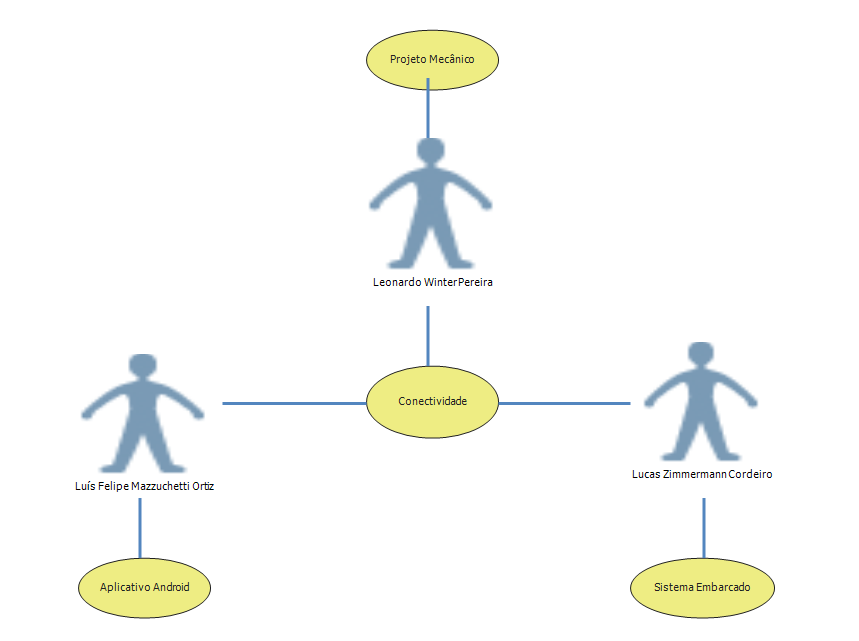
\includegraphics[scale=0.3]{Imagens/Ideia_de_projeto/equipe.png}
            \end{figure}

            \begin{itemize}
                \item Habilidades Pessoais;
            \end{itemize}

        \end{frame}

    \section{Teclado Laser}

        \begin{frame}\frametitle{Teclado Laser}

            \begin{figure}
                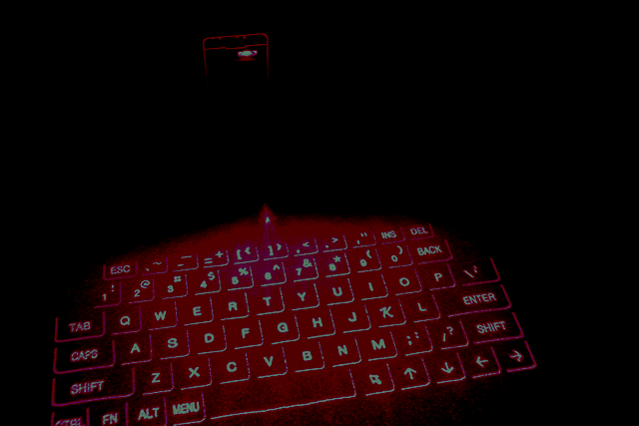
\includegraphics[scale=0.5]{Imagens/Ideia_de_projeto/teclado.png}
                \caption{Teclado Laser}
            \end{figure}

        \end{frame}

        \subsection{O que é}

             \begin{frame}\frametitle{O que é}

                \begin{itemize}
                    \item Inovação utilizando conceitos da ótica ao invés da mecânica para o evento de teclas pressionadas;
                    \item Portabilidade e adaptabilidade aumentadas em relação ao teclado mecânico;
                    \item Reconhecimento de tecla pressionada se daria pela interferência em pontos especificos de uma matriz de lasers;
                    \item Alternativamente, reconhecimento poderia se dar ao interromper o feixe entre um emissor e um receptor infravermelho, porém perdendo o aspecto visual.
                \end{itemize}

            \end{frame}

    \section{Luva Controle Remoto Universal}

        \begin{frame}\frametitle{Luva Controle Remoto Universal}

            \begin{figure}
                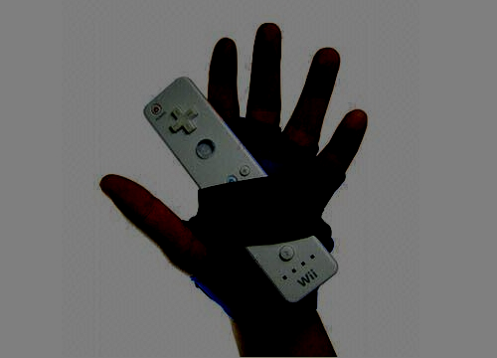
\includegraphics[scale=0.5]{Imagens/Ideia_de_projeto/luva.png}
                \caption{Luva Controle Remoto Universal}
            \end{figure}

        \end{frame}

        \subsection{O que é}

             \begin{frame}\frametitle{O que é}

                \begin{itemize}
                    \item Criação de uma luva com sensores magnéticos e/ou acelerômetros, ou ainda transmissores infravermelho;
                    \item Transmissão de comandos através do movimento das mãos e dos dedos, permite aplicações em ambientes de realidade virtual ou realidade aumentada;
                    \item Movimentos poderão ser programados através de software, e serem reconhecidos por equipamentos como computadores e aparelhos de televisão (primariamente computadores).
                \end{itemize}

            \end{frame}

    \section{Dalle Pad}

        \begin{frame}\frametitle{Dalle Pad}

            \begin{figure}
                    
\includegraphics[scale=0.35]{Imagens/Logo01.png}
                    \caption{Dalle Pad - O Gadget que te transforma em um DJ}
            \end{figure}

        \end{frame}

        \subsection{O que é}

             \begin{frame}\frametitle{O que é}

                \begin{itemize}
                    \item O DALLE PAD é um Controlador MIDI;
                    \item Mas o que é MIDI?
                \end{itemize}

                \begin{figure}
                    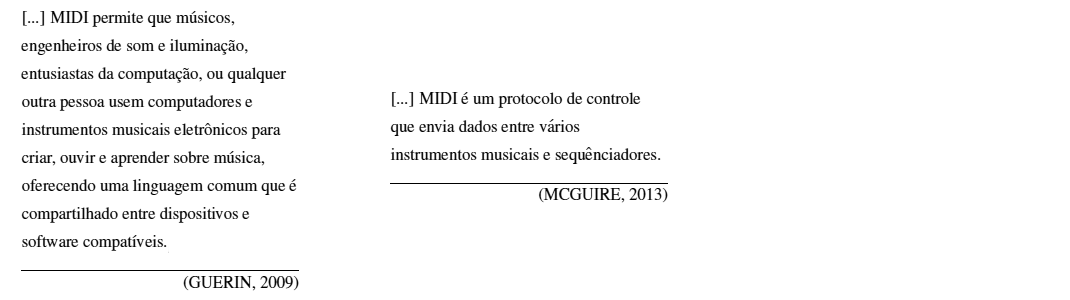
\includegraphics[scale=0.5]{Imagens/Ideia_de_projeto/epigraphs.png}
                \end{figure}

            \end{frame}

        \subsection{Ilustração do Projeto}

             \begin{frame}\frametitle{Ilustração do Projeto}

                \begin{figure}
                    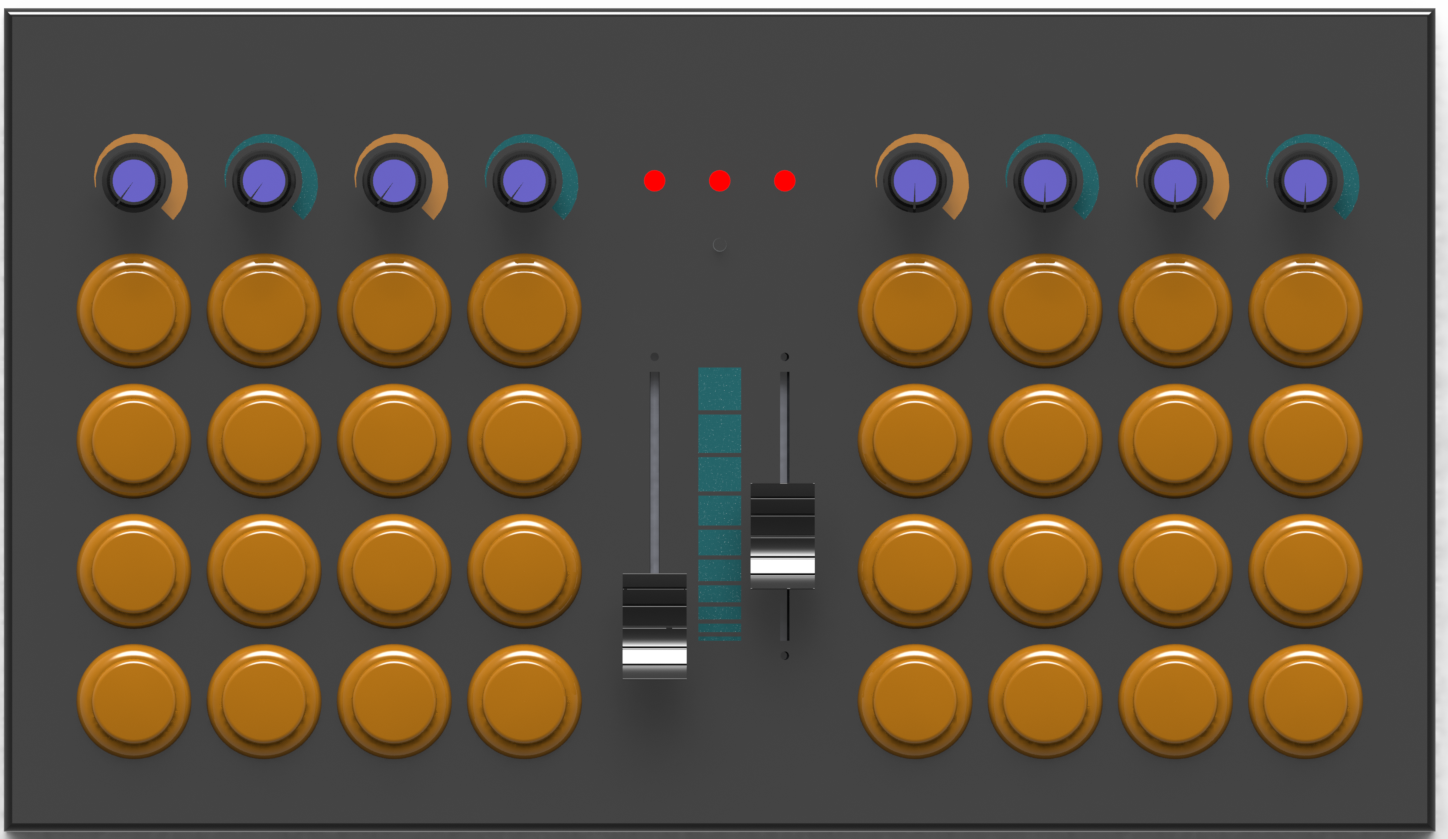
\includegraphics[scale=0.2]{Imagens/SW_Images/dalle_pad_montado2.png}
                \end{figure}

            \end{frame}

        \subsection{Partes do Projeto}

             \begin{frame}\frametitle{Partes do Projeto}

                \begin{itemize}
                    \item Projeto Mecânico;
                        \begin{figure}
                            
\includegraphics[scale=0.25]{Imagens/Ideia_de_projeto/sw.jpg}
                        \end{figure}
                    \item Sistema Embarcado;
                        \begin{figure}
                            
\includegraphics[scale=0.3]{Imagens/Ideia_de_projeto/arduino.png}
                        \end{figure}
                \end{itemize}

            \end{frame}

            \begin{frame}\frametitle{Partes do Projeto}

                \begin{itemize}
                    \item Estação Base;
                        \begin{figure}
                            
\includegraphics[scale=0.3]{Imagens/Ideia_de_projeto/android.jpg}
                        \end{figure}
                    \item Conectividade (com e sem fio):
                        \begin{figure}
                            
\includegraphics[scale=0.25]{Imagens/Ideia_de_projeto/midi_bluetooth.png}
                        \end{figure}
                \end{itemize}

            \end{frame}

        \subsection{Motivação}

            \begin{frame}\frametitle{Motivação}

                \begin{block}{Skrillex}

                    \includemovie[autoplay,showcontrols,repeat]{12cm}{6cm}{Imagens/Ideia_de_projeto/skrillex.mp4}

                \end{block}

            \end{frame}

            \begin{frame}\frametitle{Motivação}

                \begin{block}{Competição MIDI FIGHTER}
                    \includemovie[autoplay,showcontrols,repeat]{12cm}{6cm}{Imagens/Ideia_de_projeto/Arcade_Button_MIDI_Controller_Demo.mp4}

                \end{block}

            \end{frame}

\end{document} 